\documentclass[10pt,aspectratio=169]{beamer}

% --- Theme: clean default look, matching deck_overview style ---
\usetheme{default}
\setbeamertemplate{navigation symbols}{}
\setbeamertemplate{footline}{%
  \hfill\insertframenumber/\inserttotalframenumber\hspace{1em}\vspace{0.4em}}
\setbeamercolor{title}{fg=black}
\setbeamercolor{frametitle}{fg=black}
\setbeamerfont{frametitle}{series=\bfseries}
\setbeamerfont{title}{series=\bfseries, size=\Large}

% --- Packages ---
\usepackage[utf8]{inputenc}
\usepackage[T1]{fontenc}
\usepackage{graphicx}
\usepackage{booktabs}
\usepackage{tikz}
\usetikzlibrary{shapes.geometric, arrows.meta, positioning, calc}
\usepackage{xcolor}
\usepackage{amsmath}
\usepackage{amssymb}
\usepackage{tcolorbox}
\tcbuselibrary{skins}

% --- Corporate-ish palette (matches the reference Intesa-style slide) ---
\definecolor{corpblue}{RGB}{15, 56, 122}
\definecolor{corpgreen}{RGB}{30, 110, 60}
\definecolor{corporange}{RGB}{220, 130, 30}
\definecolor{corplight}{RGB}{220, 230, 245}

% --- Tableau-ish accents (consistent with deck1/deck2) ---
\definecolor{good}{RGB}{44,160,44}
\definecolor{bad}{RGB}{214,39,40}
\definecolor{warn}{RGB}{255,140,0}
\definecolor{accent}{RGB}{31,119,180}

% --- Section break helper ---
\newcommand{\mybreak}[1]{%
  \begin{frame}[plain]
    \centering
    \vspace*{\fill}
    {\LARGE\bfseries #1}
    \vspace*{\fill}
  \end{frame}}

% --- Corporate-style header panel ---
\newcommand{\panelheader}[3]{% color, title, subtitle
  \begin{tcolorbox}[
      enhanced, colback=#1, colframe=#1,
      boxrule=0pt, arc=2pt, left=10pt, right=10pt, top=6pt, bottom=6pt,
      sharp corners=southwest]
    {\color{white}\bfseries\large #2}\\[0.05cm]
    {\color{corporange}\scriptsize\bfseries\textsc{#3}}
  \end{tcolorbox}}

\title{Theme Detection via AI --- Progress \& Direction}
\subtitle{Intesa Sanpaolo AI Research --- Systematic Portfolio Management \& QIS}
\date{03 June 2026}

\begin{document}

% =====================================================================
% Slide 1 - Title
% =====================================================================
\begin{frame}[plain]
  \titlepage
  \vspace{-0.6cm}
  \centering\small
  \emph{Catching the narrative before it is priced in.}
\end{frame}


% =====================================================================
% Slide 2 - Motivations & Idea (two panels)
% =====================================================================
\begin{frame}{Motivations \& Idea}
  \footnotesize

  \begin{columns}[T,onlytextwidth]
    \column{0.49\textwidth}
      \panelheader{corpblue}{Motivation}{why thematic}
      \vspace{0.10cm}
      \begin{itemize}\setlength\itemsep{0.16cm}
        \item Sectors are a \textbf{static map} --- good for
              benchmarking, blind to change.
        \item The big moves are \textbf{cross-sector stories}
              (AI, energy transition, GLP-1 drugs).
        \item We want to catch them \textbf{early}, ahead of the index.
      \end{itemize}

    \column{0.49\textwidth}
      \panelheader{corpgreen}{Idea}{what we build}
      \vspace{0.10cm}
      \begin{itemize}\setlength\itemsep{0.16cm}
        \item \textbf{Find emerging themes automatically},
              straight from the news.
        \item No fixed list --- the news tells us what is forming.
        \item Feeds the next steps: exposure scoring and
              \textbf{baskets}.
      \end{itemize}
  \end{columns}

  \vspace{0.30cm}
  \begin{tcolorbox}[colback=corplight, colframe=corplight,
                    boxrule=0pt, arc=2pt,
                    left=10pt, right=10pt, top=5pt, bottom=5pt]
    \centering\footnotesize
    \textbf{The bet:} catch the narrative \emph{before} it is priced
    into every constituent.
  \end{tcolorbox}

\end{frame}


% =====================================================================
% Slide 3 - General schema (image only)
% =====================================================================
\begin{frame}
  \begin{center}
    \includegraphics[width=0.95\textwidth,height=0.92\textheight,keepaspectratio]%
      {general-schema.png}
  \end{center}
\end{frame}


% =====================================================================
% Slide 4 - Taxonomy
% =====================================================================
\begin{frame}{Taxonomy --- what counts as a theme}
  \footnotesize

  \textbf{Granularity ladder.}\;
  News carries events; events recur into themes; a theme plus exposure
  becomes tradable.

  \vspace{0.10cm}
  \begin{center}
  \resizebox{0.92\textwidth}{!}{%
  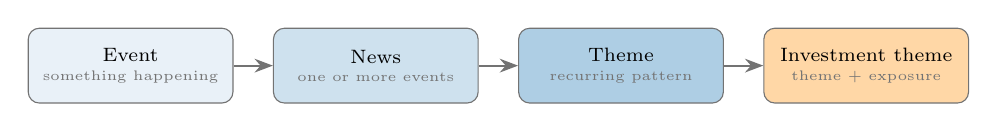
\begin{tikzpicture}[
      node distance=0.1cm,
      box/.style={rectangle, rounded corners, draw=black!55, line width=0.4pt,
                  minimum width=2.6cm, minimum height=0.95cm,
                  font=\scriptsize, align=center},
      arr/.style={-Stealth, thick, draw=black!55}
    ]
    \node[box, fill=accent!10] (e) {Event\\[-0.05cm]\textcolor{black!55}{\tiny something happening}};
    \node[box, fill=accent!22, right=0.50cm of e] (n) {News\\[-0.05cm]\textcolor{black!55}{\tiny one or more events}};
    \node[box, fill=accent!36, right=0.50cm of n] (t) {Theme\\[-0.05cm]\textcolor{black!55}{\tiny recurring pattern}};
    \node[box, fill=warn!35,   right=0.50cm of t] (i) {Investment theme\\[-0.05cm]\textcolor{black!55}{\tiny theme + exposure}};
    \draw[arr] (e) -- (n);
    \draw[arr] (n) -- (t);
    \draw[arr] (t) -- (i);
  \end{tikzpicture}}
  \end{center}

  \vspace{0.15cm}
  \begin{tcolorbox}[colback=corpblue!8, colframe=corpblue,
                    boxrule=0.4pt, arc=2pt,
                    left=8pt, right=8pt, top=4pt, bottom=4pt]
    \footnotesize
    \textbf{What is a theme?}\; It is \textbf{transient} (it has a
    lifecycle) and \textbf{cross-sector} (it links firms that sectors keep apart).
  \end{tcolorbox}

  \vspace{0.15cm}
  \textbf{Lifecycle --- target window: emerging $\rightarrow$ validated.}
  \begin{center}
  \resizebox{0.98\textwidth}{!}{%
  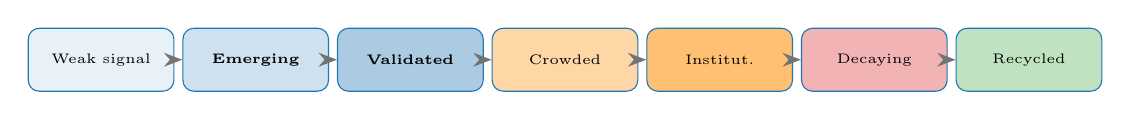
\begin{tikzpicture}[
      node distance=0.05cm,
      stage/.style={rectangle, rounded corners, draw=accent, line width=0.4pt,
                    minimum width=1.85cm, minimum height=0.80cm,
                    font=\tiny, align=center},
      arr/.style={-Stealth, thick, draw=black!55}
    ]
    \node[stage, fill=accent!10] (a) {Weak signal};
    \node[stage, fill=accent!22, right=0.10cm of a] (b) {\textbf{Emerging}};
    \node[stage, fill=accent!38, right=0.10cm of b] (c) {\textbf{Validated}};
    \node[stage, fill=warn!35,   right=0.10cm of c] (d) {Crowded};
    \node[stage, fill=warn!55,   right=0.10cm of d] (e2) {Institut.};
    \node[stage, fill=bad!35,    right=0.10cm of e2] (f) {Decaying};
    \node[stage, fill=good!30,   right=0.10cm of f] (g) {Recycled};
    \draw[arr] (a) -- (b);
    \draw[arr] (b) -- (c);
    \draw[arr] (c) -- (d);
    \draw[arr] (d) -- (e2);
    \draw[arr] (e2) -- (f);
    \draw[arr] (f) -- (g);
  \end{tikzpicture}}
  \end{center}

\end{frame}


% =====================================================================
% Slide 4 - The data
% =====================================================================
\begin{frame}{The data}
  \footnotesize

  \begin{columns}[T,onlytextwidth]
    \column{0.49\textwidth}
      \panelheader{corpblue}{News corpus}{the signal source}
      \vspace{0.10cm}
      \begin{itemize}\setlength\itemsep{0.10cm}
        \item Bloomberg wire, \texttt{raw\_news\_2025.csv} ---
              \textbf{8.9\,GB}, from 2025, \textbf{$\sim$50k articles/day}.
        \item Each story carries \textbf{tickers},
              \textbf{$\sim$1{,}800 Bloomberg topic codes}, wire \& event type.
        \item Heavy duplication (versions / re-issues) ---
              de-duplicated before use.
      \end{itemize}

    \column{0.49\textwidth}
      \panelheader{corpgreen}{Thematic ETF panel}{the market anchor}
      \vspace{0.10cm}
      \begin{itemize}\setlength\itemsep{0.10cm}
        \item \textbf{27 thematic ETFs} (AI, nuclear, quantum, space,
              clean energy, cyber, EV, \dots).
        \item Daily \textbf{price, fund flow, volume},
              \textbf{2018--2026} ($\sim$1{,}980 trading days).
        \item Define the theme list \emph{and} give a market-side
              benchmark to validate against.
      \end{itemize}
  \end{columns}

  \vspace{0.20cm}
  \begin{tcolorbox}[colback=warn!12, colframe=warn,
                    boxrule=0.4pt, arc=2pt, left=8pt, right=8pt, top=4pt, bottom=4pt]
    \footnotesize
    \textbf{Early finding:} theme coverage is very skewed --- Tech \&
    Communications tags $\sim$99\% of articles, while Quantum, Cyber and
    Cannabis are under 5\%. Motivates de-duplication, top-$k$ tagging,
    and unsupervised discovery.
  \end{tcolorbox}

\end{frame}


% =====================================================================
% Slide 5 - Data: Input -> Output
% =====================================================================
\begin{frame}{Data --- input $\rightarrow$ output}
  \footnotesize

  \textbf{Input (three tiers).}
  \vspace{0.10cm}
  \begin{center}
  \resizebox{0.97\textwidth}{!}{%
  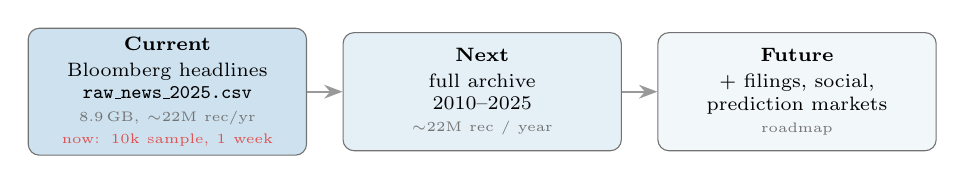
\begin{tikzpicture}[
      node distance=0.1cm,
      box/.style={rectangle, rounded corners, draw=black!55, line width=0.4pt,
                  minimum width=3.5cm, minimum height=1.5cm,
                  font=\scriptsize, align=center, text width=3.3cm},
      arr/.style={-Stealth, thick, draw=black!40}
    ]
    \node[box, fill=accent!22] (cur)
      {\textbf{Current}\\[0.05cm]Bloomberg headlines\\\texttt{raw\_news\_2025.csv}\\
       \textcolor{black!55}{\tiny 8.9\,GB, $\sim$22M rec/yr}\\
       \textcolor{bad!80}{\tiny now: 10k sample, 1 week}};
    \node[box, fill=accent!12, right=0.45cm of cur] (nxt)
      {\textbf{Next}\\[0.05cm]full archive\\2010--2025\\
       \textcolor{black!55}{\tiny $\sim$22M rec / year}};
    \node[box, fill=accent!6, right=0.45cm of nxt] (fut)
      {\textbf{Future}\\[0.05cm]+ filings, social,\\prediction markets\\
       \textcolor{black!55}{\tiny roadmap}};
    \draw[arr] (cur) -- (nxt);
    \draw[arr] (nxt) -- (fut);
  \end{tikzpicture}}
  \end{center}

  \vspace{0.10cm}
  \textit{Transform:} strip wire prefixes \& dates $\rightarrow$
  finance-domain embeddings.

  \vspace{0.15cm}
  \textbf{Output (ideal target --- not yet formulated).}\;
  Ranked themes \emph{tracked over time}, each tagged with nearest ICB
  sector + similarity, split aligned / novel:
  \begin{center}
  \resizebox{0.80\textwidth}{!}{%
  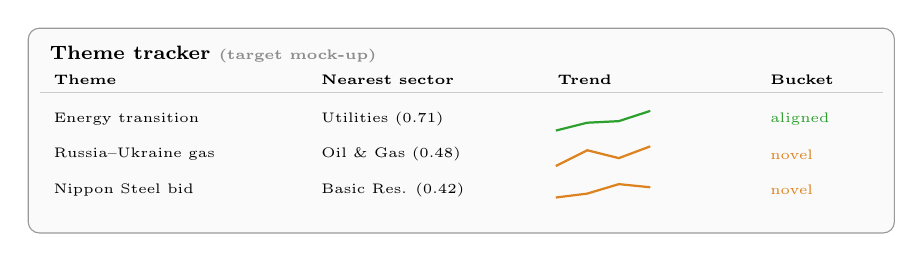
\begin{tikzpicture}[font=\scriptsize]
    % dashboard frame
    \draw[draw=black!40, rounded corners, fill=black!2] (0,0) rectangle (11,2.6);
    \node[anchor=north west, font=\scriptsize\bfseries] at (0.15,2.5)
      {Theme tracker \textcolor{black!45}{\tiny (target mock-up)}};
    % column headers
    \node[anchor=west, font=\tiny\bfseries] at (0.2,1.95) {Theme};
    \node[anchor=west, font=\tiny\bfseries] at (3.6,1.95) {Nearest sector};
    \node[anchor=west, font=\tiny\bfseries] at (6.6,1.95) {Trend};
    \node[anchor=west, font=\tiny\bfseries] at (9.3,1.95) {Bucket};
    \draw[black!20] (0.15,1.78) -- (10.85,1.78);
    % rows
    \node[anchor=west, font=\tiny] at (0.2,1.45) {Energy transition};
    \node[anchor=west, font=\tiny] at (3.6,1.45) {Utilities (0.71)};
    \draw[good, thick] (6.7,1.30) -- (7.1,1.40) -- (7.5,1.42) -- (7.9,1.55);
    \node[anchor=west, font=\tiny, text=good] at (9.3,1.45) {aligned};
    \node[anchor=west, font=\tiny] at (0.2,1.00) {Russia--Ukraine gas};
    \node[anchor=west, font=\tiny] at (3.6,1.00) {Oil \& Gas (0.48)};
    \draw[corporange, thick] (6.7,0.85) -- (7.1,1.05) -- (7.5,0.95) -- (7.9,1.10);
    \node[anchor=west, font=\tiny, text=corporange] at (9.3,1.00) {novel};
    \node[anchor=west, font=\tiny] at (0.2,0.55) {Nippon Steel bid};
    \node[anchor=west, font=\tiny] at (3.6,0.55) {Basic Res. (0.42)};
    \draw[corporange, thick] (6.7,0.45) -- (7.1,0.50) -- (7.5,0.62) -- (7.9,0.58);
    \node[anchor=west, font=\tiny, text=corporange] at (9.3,0.55) {novel};
  \end{tikzpicture}}
  \end{center}

\end{frame}


% =====================================================================
% Slide 5 - Pipeline (with approach landscape)
% =====================================================================
\begin{frame}{Pipeline --- where we are, and the approach landscape}
  \footnotesize

  \textbf{Three-stage spine.}
  \begin{center}
  \resizebox{0.85\textwidth}{!}{%
  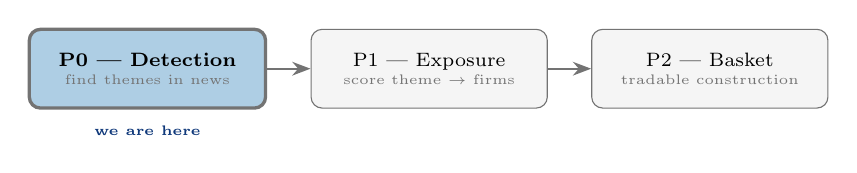
\begin{tikzpicture}[
      node distance=0.1cm,
      box/.style={rectangle, rounded corners, draw=black!55, line width=0.4pt,
                  minimum width=3.0cm, minimum height=1.0cm,
                  font=\scriptsize, align=center},
      arr/.style={-Stealth, thick, draw=black!55}
    ]
    \node[box, fill=accent!36, line width=1.2pt] (p0)
      {\textbf{P0 --- Detection}\\[-0.05cm]\textcolor{black!55}{\tiny find themes in news}};
    \node[box, fill=black!4, right=0.55cm of p0] (p1)
      {P1 --- Exposure\\[-0.05cm]\textcolor{black!55}{\tiny score theme $\to$ firms}};
    \node[box, fill=black!4, right=0.55cm of p1] (p2)
      {P2 --- Basket\\[-0.05cm]\textcolor{black!55}{\tiny tradable construction}};
    \draw[arr] (p0) -- (p1);
    \draw[arr] (p1) -- (p2);
    \node[below=0.08cm of p0, font=\tiny\bfseries, text=corpblue] {we are here};
  \end{tikzpicture}}
  \end{center}

  \vspace{0.15cm}
  \textbf{Approach landscape} (high level; \textbf{our choice in bold}):
  \vspace{0.05cm}
  \begin{columns}[T,onlytextwidth]
    \column{0.49\textwidth}
      \begin{itemize}\setlength\itemsep{0.05cm}
        \item \emph{Discovery, classical:} LDA, NMF
        \item \emph{Discovery, embedding/neural:}
              \textbf{BERTopic (ours)}, Top2Vec
        \item \emph{Short-text:} embedding clustering, LLM labeling
      \end{itemize}
    \column{0.49\textwidth}
      \begin{itemize}\setlength\itemsep{0.05cm}
        \item \emph{Temporal/streaming:} RollingLDA, BERTopic-over-time
        \item \emph{Exposure scoring:} keyword rules, revenue mapping,
              embedding similarity, LLM classification
      \end{itemize}
  \end{columns}

  \vspace{0.15cm}
  \begin{tcolorbox}[colback=corplight, colframe=corplight,
                    boxrule=0pt, arc=2pt, left=8pt, right=8pt, top=4pt, bottom=4pt]
    \footnotesize
    \textit{Exposure scoring} = how strongly each company's cash flows are
    tied to the theme --- the bridge from P0 detection to P1.
  \end{tcolorbox}

\end{frame}


% =====================================================================
% Slide 6 - Progression (done / current results)
% =====================================================================
\begin{frame}{Progression --- done \& current results}
  \footnotesize

  \begin{columns}[T,onlytextwidth]
    \column{0.50\textwidth}
      \textbf{\textcolor{corpgreen}{Done --- end-to-end P0 prototype.}}
      \vspace{0.10cm}
      \begin{center}
      \resizebox{\textwidth}{!}{%
      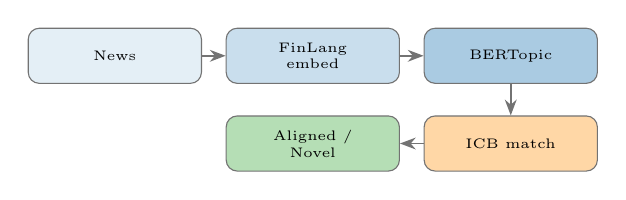
\begin{tikzpicture}[
          node distance=0.1cm,
          box/.style={rectangle, rounded corners, draw=black!55, line width=0.4pt,
                      minimum width=2.2cm, minimum height=0.7cm,
                      font=\tiny, align=center},
          arr/.style={-Stealth, semithick, draw=black!55}
        ]
        \node[box, fill=accent!12] (n) {News};
        \node[box, fill=accent!24, right=0.30cm of n] (e) {FinLang\\embed};
        \node[box, fill=accent!38, right=0.30cm of e] (c) {BERTopic};
        \draw[arr] (n) -- (e);
        \draw[arr] (e) -- (c);
        \node[box, fill=warn!35, below=0.40cm of c] (m) {ICB match};
        \node[box, fill=good!35, left=0.30cm of m] (o) {Aligned /\\Novel};
        \draw[arr] (c) -- (m);
        \draw[arr] (m) -- (o);
      \end{tikzpicture}}
      \end{center}
      \vspace{0.05cm}
      News $\rightarrow$ FinLang embeddings $\rightarrow$ BERTopic
      $\rightarrow$ ICB sector matching $\rightarrow$ aligned/novel ranking,
      with Sankey drill-down.

    \column{0.50\textwidth}
      \textbf{Current results} \textcolor{black!55}{\scriptsize (10k sample, one week)}
      \begin{itemize}\setlength\itemsep{0.05cm}
        \item \textbf{Around 40 themes} matched against the ICB sectors.
        \item Split into \textbf{aligned} / \textbf{novel} buckets.
      \end{itemize}
      \vspace{0.10cm}
      \begin{tcolorbox}[colback=black!3, colframe=black!20,
                        boxrule=0.4pt, arc=2pt, left=6pt, right=6pt, top=3pt, bottom=3pt]
        \scriptsize
        \textcolor{good}{\textbf{Aligned:}} oil \& gas, EV / auto.\\[0.10cm]
        \textcolor{corporange}{\textbf{Novel candidates:}}
        Russia--Ukraine gas, Nippon Steel bid.\\[0.10cm]
        \textcolor{bad}{\textbf{Single-event noise:}}
        Cybertruck, New Orleans.
      \end{tcolorbox}
      \vspace{0.05cm}
      \textcolor{black!55}{\scriptsize The novel bucket is the interesting one ---
      cross-sector / transient candidates.}
  \end{columns}

\end{frame}


% =====================================================================
% Slide 7 - Time -> Resources
% =====================================================================
\begin{frame}{Time $\rightarrow$ resources}
  \footnotesize

  \textbf{Measured on this laptop} \textcolor{black!55}{\scriptsize (Apple Silicon, MPS;
  real embed + cluster pipeline)}.

  \begin{columns}[T,onlytextwidth]
    \column{0.52\textwidth}
      \textbf{\textcolor{corpblue}{Now --- laptop}}
      \begin{itemize}\setlength\itemsep{0.04cm}
        \item Detection (embed + cluster):
              \textbf{$\sim$1 day per year} of news.
        \item Sentiment, light \textcolor{black!55}{\scriptsize(FinBERT-class)}:
              $\sim$650 headlines/s $\to$ \textbf{$\sim$3--4 h / year}.
        \item Sentiment, LLM \textcolor{black!55}{\scriptsize(7B, generative)}:
              $\sim$2.6 headlines/s $\to$ \textcolor{bad}{\textbf{$\sim$36 days / year}}.
        \item Memory wall: 1 yr $\approx$ 25\,GB of embeddings;
              multi-year ($\sim$130M) $\to$ must stream / out-of-core.
      \end{itemize}

    \column{0.46\textwidth}
      \textbf{\textcolor{corpgreen}{With GPU --- A100-class}}
      \begin{itemize}\setlength\itemsep{0.04cm}
        \item Detection $\sim$10--30$\times$ faster;
              full multi-year archive becomes routine.
        \item Headroom for clustering at scale (no RAM wall).
        \item \textbf{LLM sentiment / exposure: $\sim$36 days $\to$ hours}
              per year via batched serving ($\sim$100$\times$).
      \end{itemize}
      \vspace{0.10cm}
      \begin{tcolorbox}[colback=corplight, colframe=corplight,
                        boxrule=0pt, arc=2pt, left=6pt, right=6pt, top=3pt, bottom=3pt]
        \scriptsize
        \textbf{Asks:} A100 GPU node ($\sim$EUR\,17k/yr), storage,
        LLM licenses. POC $\sim$EUR\,12--16k over 6--8 months.
      \end{tcolorbox}
  \end{columns}

  \vspace{0.15cm}
  \begin{tcolorbox}[colback=corpblue!8, colframe=corpblue,
                    boxrule=0.4pt, arc=2pt, left=8pt, right=8pt, top=4pt, bottom=4pt]
    \centering\footnotesize
    \textbf{We are compute-bound, not idea-bound} --- the GPU unlocks full
    coverage \emph{and} the LLM sentiment / exposure layer.
  \end{tcolorbox}

\end{frame}


% =====================================================================
% Slide 8 - Next steps
% =====================================================================
\begin{frame}{Next steps}
  \footnotesize

  \begin{columns}[T,onlytextwidth]
    \column{0.49\textwidth}
      \panelheader{corpblue}{Time analysis of themes}{temporal tracking}
      \vspace{0.10cm}
      \begin{itemize}\setlength\itemsep{0.08cm}
        \item Move from a \textbf{static snapshot} to \textbf{online
              temporal tracking}.
        \item Detect continuation / split / merge / birth of themes.
        \item Catch themes at the \textbf{emerging} stage; filter
              single-event noise.
      \end{itemize}

    \column{0.49\textwidth}
      \panelheader{corpgreen}{Validation}{does it work}
      \vspace{0.10cm}
      \begin{itemize}\setlength\itemsep{0.08cm}
        \item Worked example: \textbf{AI theme} --- confirm the system
              would surface it \emph{before} the AI-themed ETFs launched
              (the ``validated'' stage).
        \item Metrics: topic coherence (NPMI, $C_v$), ranking vs ETF
              benchmarks, factor neutrality, guardrails vs thematic
              illusions.
      \end{itemize}
  \end{columns}

  \vspace{0.25cm}
  \begin{tcolorbox}[colback=corplight, colframe=corplight,
                    boxrule=0pt, arc=2pt, left=10pt, right=10pt, top=4pt, bottom=4pt]
    \footnotesize
    \textbf{Secondary track:}\;
    better embeddings (FinBERT-MPNet / LoRA-bge-large)
    \quad\textbullet\quad
    theme $\rightarrow$ exposure mapping (toward P1) \textbullet \quad additional heterogeneous data sources.
  \end{tcolorbox}

\end{frame}


\end{document}
